\textbf{TODO: Summary by Anton}
%%% Local Variables:
%%% mode: latex
%%% TeX-master: "../../report"
%%% End:
\begin{figure}[h]
    \centering
    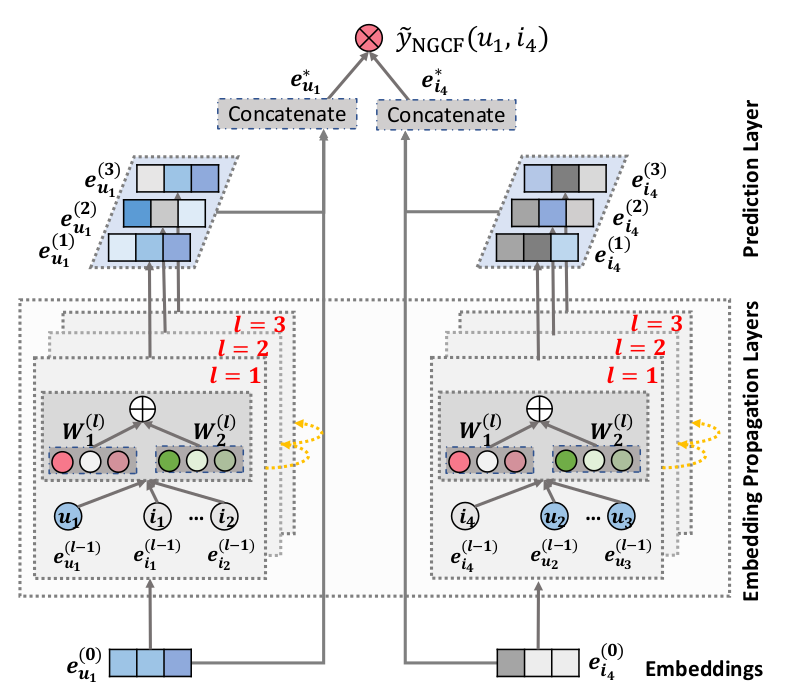
\includegraphics[width=0.8\linewidth]{images/ngcf.png}
    \caption{NGCF architecture.}
    \label{fig:ngcf}
\end{figure}

Tha main difference of NGCF \cite{wang2019neural} from NCF is the embedding propagation layers which are 
designed to incorporate collaborative signal, including high-order connectivities 
in users-items connections graph, into embeddings of users and items \ref{fig:ngcf}.
Therefore, this is supposed toimprove the quality of recommendations. 

Each layer corresponds to specific length of path from between user and item.
It produces messages which are passed between these nodes, summed and result in
embedding at this level. All embeddings from all levels are in the end concatenated
producing final embeddding.
These embeddings play roles of latent vectors which can be simply multiplied 
in order to obtain resulting rating.
Model is trained using pairwise BPR loss and mini--batch Adam optimizer.